
We present a geometric framework for semantic invariance in language models, based on the hypothesis that paraphrastic variation induces structured zones of stability. Section~\ref{sec: define} formalizes invariant latent features, Section~\ref{sec: find} introduces a contrastive subspace discovery method, and Section~\ref{sec: attribution_app} uses the resulting representations for zero-shot model attribution as empirical validation.

\subsection{Invariant Latent Features: Definition and Local Geometry}
\label{sec: define}

Let \(f_m\) denote a language model, \(h_\ell(x)\in\mathbb{R}^{T\times d}\) denote the token-level hidden states at layer \(\ell\), and \(z=\Phi_\ell(x)\in\mathbb{R}^d\) denote their pooled representation, which serves as the primary object of analysis. 
We study invariance of these representations under semantic-preserving transformations. Formally, for a transformation \(T(\cdot)\) such as paraphrasing, invariance requires
\(
\Phi_\ell(T(x)) \approx \Phi_\ell(x).
\)
To avoid trivial collapse, representations must also remain discriminative across meanings. Specifically, for paraphrases \(x_1,x_2\) and an input \(x_3\) with different meaning, we require
\(
\Phi_\ell(x_1) \approx \Phi_\ell(x_2), \quad
\Phi_\ell(x_1) \not\approx \Phi_\ell(x_3).
\)
This within--between criterion defines invariant latent features as representations that are stable under semantic-preserving variation while remaining separable across semantic content. 

To interpret this property, we adopt a geometric perspective inspired by the manifold hypothesis~\cite{fefferman2016testing}. Although latent representations reside in a high-dimensional ambient space \(\mathbb{R}^d\), meaningful semantic information occupies only a structured subset of this space. Let \(\mathcal{M} \subset \mathbb{R}^d\) denote the semantic representation manifold. Inputs with coherent semantic meaning are mapped to points lying near this manifold, while arbitrary points in the ambient space generally do not correspond to meaningful language representations. 
Under this view, semantically equivalent inputs correspond to nearby points on the manifold. Paraphrasing can therefore be interpreted as a local perturbation that moves the representation within a neighborhood of the same semantic region. Specifically, for paraphrases \(x_1\) and \(x_2\),
\(
\|\Phi_\ell(x_1) - \Phi_\ell(x_2)\| \leq \epsilon,
\)
for some small \(\epsilon > 0\), while input \(x_3\) with distinct semantic meaning occupy separate regions of the manifold.

We propose to analyze the local structure of \(\mathcal{M}\) through its tangent space. At a point \(z=\Phi_\ell(x)\) on the manifold, the tangent space \(T_z\mathcal{M}\) contains all directions along which the representation can move infinitesimally while remaining on the manifold. In other words, \(T_z\mathcal{M}\) provides a local linear approximation of the manifold and captures the allowable directions of variation in representation space. 
Figure~\ref{fig:define} illustrates this local geometric interpretation. Variations of representations on the manifold arise from two qualitatively different sources: semantic changes, which alter the underlying meaning of the input, and nuisance changes, which modify surface form while preserving semantic content. 
Locally, these two types of variation can be interpreted as approximately distinct directions within the tangent space. We therefore consider a working decomposition of the form
\begin{equation}
T_z\mathcal{M} \approx T_z^{\mathrm{semantic}} \cup T_z^{\mathrm{nuisance}}
\label{eq: tan_decompose}
\end{equation}
where $T^{\text{semantic}}_z$ captures directions associated with changes in semantic content, and $T^{\text{nuisance}}_z$ captures directions corresponding to semantic-preserving variation. In practice, this decomposition is a local and approximate factorization, since learned representations may exhibit partial overlap and entanglement between these components. 
% Locally, these two types of variation can be interpreted as distinct directions within the tangent space,
% \begin{equation}
%     T_z \mathcal{M} \approx T^{\text{semantic}}_z \oplus T^{\text{nuisance}}_z .
% \label{eq: tan_decompose}
% \end{equation}
Under a semantic-preserving transformation such as paraphrasing, the representation primarily moves along nuisance directions,
\(
z' = z + v_{\text{nuisance}} .
\)
Invariant features correspond to representations that ignore such nuisance motion. If \(P\) denotes a projection operator onto the semantic subspace, the invariant representation can be written as
\(
z_{\text{inv}} = Pz,
\)
which satisfies
\(
P(z + v_{\text{nuisance}}) = Pz.
\)
% Intuitively, invariant features preserve semantic identity while removing variation caused by surface-level transformations.
Throughout this work, ``invariant'' refers specifically to invariance with respect to semantic-preserving transformations. Thus, invariant features are expected to remain stable under paraphrasing while remaining sensitive to semantic-changing perturbations.

\begin{wrapfigure}{r}{0.70\textwidth}
  \centering
  \vspace{-1.0em}
  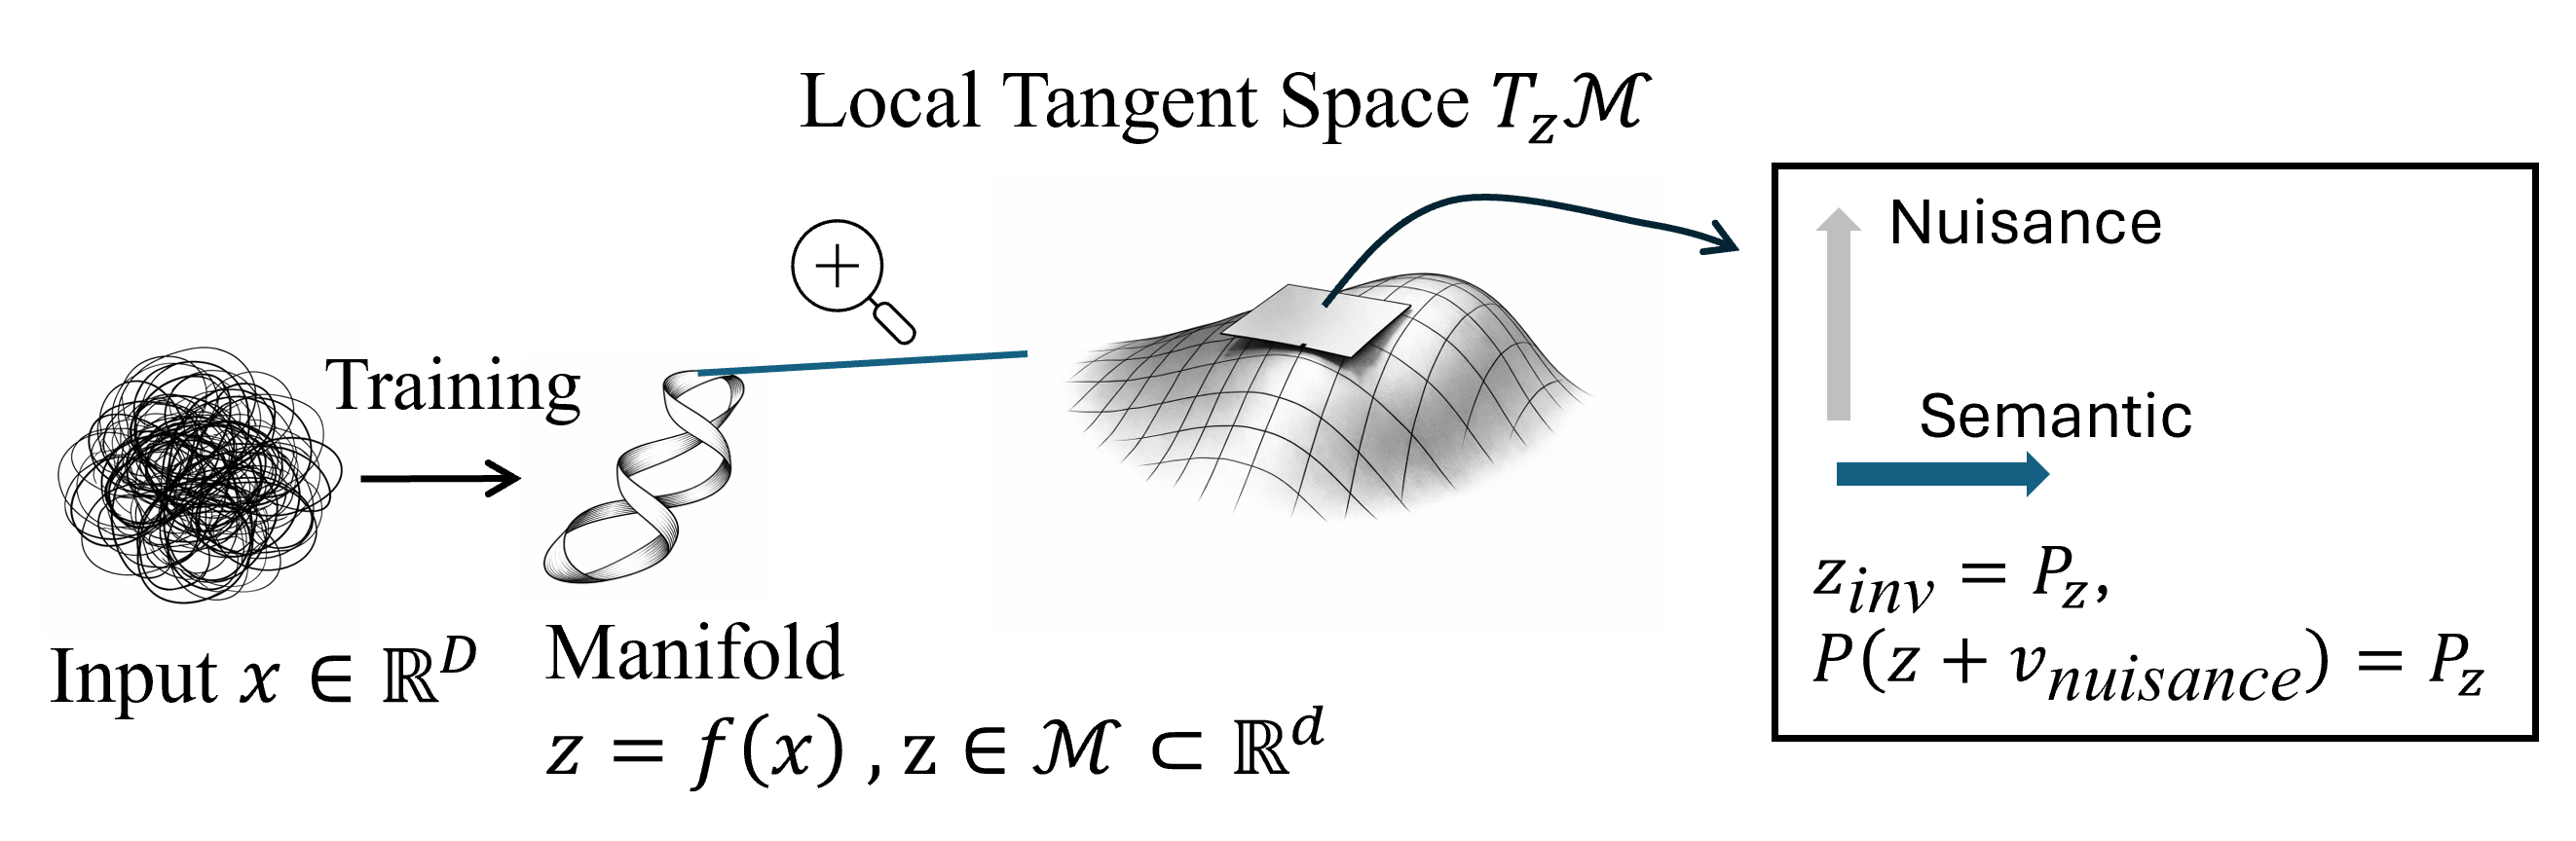
\includegraphics[width=1.0\linewidth]{figures/2_Define.png}
  \vspace{-2.0em}
  \caption{
    Local geometric hypothesis of semantic invariance in LM representations. 
    During training, inputs $x \in \mathbb{R}^D$ are mapped by the model to latent representations 
    $z = f(x)$ that lie on a lower-dimensional manifold $\mathcal{M} \subset \mathbb{R}^d$. 
    At a point $z \in \mathcal{M}$, the tangent space $T_z\mathcal{M}$ provides a local linear 
    approximation of allowable variations in representation space. 
    Semantic-preserving transformations such as paraphrasing primarily induce movements along 
    nuisance directions that do not alter the underlying meaning. 
    Invariant latent features correspond to projections that remove these nuisance directions, 
    so that $z_{\text{inv}} = P_z$ and $P(z + v_{\text{nuisance}}) = P_z$, preserving semantic identity 
    while ignoring surface variation.
    }
  \label{fig:define}
  \vspace{-1.0em}
\end{wrapfigure}

This local geometric interpretation provides an explanation for why invariant latent features naturally emerge during training. To maintain consistent behavior under paraphrasing, the model must map semantically equivalent inputs to nearby regions in latent space while preserving separability across meanings. These constraints induce structured zones of stability on the representation manifold where paraphrase variants cluster while remaining distinguishable from other semantic concepts.

Although the existence of such invariant zones follows from the need for semantic consistency, their geometric realization is generally model-specific. Transformer training involves highly non-convex optimization~\cite{kawaguchi2016deep, choromanska2015loss}, and different models may converge to distinct embeddings of the underlying semantic manifold due to variations in initialization, architecture, training data, and optimization dynamics. Consequently, even when two models encode similar semantic concepts, the corresponding latent manifolds may differ in orientation, curvature, and local geometry. Invariant latent features therefore reflect how a particular model internally organizes semantic information. This combination of semantic stability and geometric individuality later enables these invariant representations to serve as distinctive identifiers for model attribution.


\subsection{Invariant Subspace Identification via Contrastive Sensitivity Decomposition}
\label{sec: find}

The geometric formulation in Section~\ref{sec: define} characterizes invariant latent features as directions that remain stable under semantic-preserving transformations while remaining responsive to semantic change. We now introduce a data-driven procedure to identify such directions from model activations. The key idea is to contrast two sources of variation in latent space: variation induced by semantic-preserving transformations, which primarily reflects nuisance motion, and variation induced by semantic-changing transformations, which reflects movement across meanings.

Let \(x\) denote an input prompt, at layer $\ell$, let $h_\ell(x) \in \mathbb{R}^{T \times d}$ denote token-level hidden states. We define a representation vector $z_\ell(x)=\Phi_\ell(x)\in\mathbb{R}^d$ as a deterministic pooling of $h_\ell(x)$. 
In practice, we use the final-token hidden state, i.e., $z_\ell(x)=h_\ell^{(T)}(x)$, which incorporates information from preceding tokens and directly supports next-token prediction. We compare this choice with mean pooling in Appendix~\ref{app:pooling}.
For each input, we construct two perturbation families. The first consists of semantic-preserving variants, denoted by \(\{x_i^{\mathrm{sp}}\}_{i=1}^{n}\), such as paraphrases that preserve the underlying meaning while altering surface form. The second consists of semantic-changing variants, denoted by \(\{x_j^{\mathrm{sc}}\}_{j=1}^{m}\), whose semantic content differs from that of the anchor input. We then compute the corresponding finite-difference feature changes
\(
\Delta z_i^{\mathrm{sp}}=\Phi_\ell(x_i^{\mathrm{sp}})-\Phi_\ell(x),
\)
\(
\Delta z_j^{\mathrm{sc}}=\Phi_\ell(x_j^{\mathrm{sc}})-\Phi_\ell(x).
\)
These difference vectors provide empirical estimates of local motion in the representation space. Under the local geometric hypothesis, semantic-preserving perturbations primarily trace nuisance directions in the tangent space, whereas semantic-changing perturbations additionally traverse semantic directions. To capture these two modes of variation, we define the empirical sensitivity covariances
\(
S_{\ell}^{\mathrm{sp}}=
\frac{1}{n}\sum_{i=1}^{n}\Delta z_i^{\mathrm{sp}}(\Delta z_i^{\mathrm{sp}})^\top,
\)
\(
S_{\ell}^{\mathrm{sc}}=
\frac{1}{m}\sum_{j=1}^{m}\Delta z_j^{\mathrm{sc}}(\Delta z_j^{\mathrm{sc}})^\top.
\) 
We then identify contrastive directions by solving the generalized eigenvalue problem:
\begin{equation}
   S_{\ell}^{\mathrm{sc}} v = \lambda \, S_{\ell}^{\mathrm{sp}} v. 
\label{eq: cross_eigen}
\end{equation}
Each eigenvector \(v\) maximizes the Rayleigh quotient
\(
\lambda(v)=
v^\top S_{\ell}^{\mathrm{sc}} v / v^\top S_{\ell}^{\mathrm{sp}} v.
\)
% \[
% \lambda(v)=
% \frac{v^\top S_{\ell}^{\mathrm{sc}} v}
%      {v^\top S_{\ell}^{\mathrm{sp}} v}.
% \]
This formulation encodes the desired notion of the proposed invariance. 
Directions with large \(\lambda\) exhibit strong variation under semantic change but weak variation under semantic-preserving perturbations, and therefore correspond to invariant semantic directions. In contrast, directions with small \(\lambda\) are dominated by semantic-preserving variation and are interpreted as nuisance directions. 
% Thus, invariant directions are those that are small under semantic-preserving perturbations yet large under semantic-changing perturbations, whereas nuisance directions are highly sensitive to semantic-preserving transformations. 
We therefore use the term invariant direction to denote a direction that is stable under semantic-preserving perturbations but discriminative under semantic-changing perturbations. 
All covariance estimates and the generalized eigenvalue problem are computed on $z_\ell(x)$.

In practice, $S_{\mathrm{sp}}$ is low rank because the number of semantic-preserving perturbations is much smaller than the hidden dimension. We therefore solve a regularized generalized eigenvalue problem, which ensures positive definiteness of the denominator operator and yields a well-posed decomposition,
\(
S_{\mathrm{sc}} v = \lambda (S_{\mathrm{sp}} + \epsilon I)v,
\)
where $\epsilon > 0$ ensures numerical stability. Let $V_{\ell}^{\mathrm{inv}} = [v_1, \ldots, v_k]$ denote the top-$k$ generalized eigenvectors with the largest eigenvalues at layer $\ell$. 
Since generalized eigenvectors are orthogonal with respect to the $(S_{\mathrm{sp}} + \epsilon I)$-inner product but not necessarily under the Euclidean inner product, we compute an orthonormal basis
\(
U_\ell^{\mathrm{inv}} = \mathrm{orth}(V_\ell^{\mathrm{inv}})
\)
via QR decomposition. This ensures that $U_\ell^{\mathrm{inv}} U_\ell^{\mathrm{inv}\top}$ defines a valid Euclidean projection operator. 
The invariant representation at layer $\ell$ is then obtained by projection,
\begin{equation}
z_{\mathrm{inv}}
=
U_\ell^{\mathrm{inv}}
U_\ell^{\mathrm{inv}\top} z .
\label{eq: decompose_z_inv}
\end{equation}
This projection suppresses nuisance-sensitive components while preserving directions that remain stable under paraphrasing yet discriminate across meanings. 
The complementary nuisance component is given by
\(
z_{\mathrm{nuis}}
=
\left(
I-
U_\ell^{\mathrm{inv}}
U_\ell^{\mathrm{inv}\top}
\right) z.
\)
Together they induce the decomposition
\(
z = z_{\mathrm{inv}} + z_{\mathrm{nuis}},
\)
providing a constructive approximation of the semantic--nuisance decomposition in Eq.~\ref{eq: tan_decompose}. In particular, \(z_{\mathrm{inv}}\) captures components aligned with invariant semantic directions, while \(z_{\mathrm{nuis}}\) captures variation dominated by nuisance-sensitive directions.

The decomposition in Eq.~\ref{eq: decompose_z_inv} also admits a local differential interpretation. When perturbations are infinitesimal, \(\Delta z \approx J_{\Phi_\ell}(x)\Delta x\), where \(J_{\Phi_\ell}(x)\) is the Jacobian of the layer-wise representation map. The resulting covariance operators satisfy
\(
S \approx J_{\Phi_\ell}(x)\,\mathbb{E}[\Delta x \Delta x^\top]\,J_{\Phi_\ell}(x)^\top.
\)
Hence, the proposed covariance-based formulation can be viewed as a data-driven approximation of Jacobian sensitivity. Moreover, if the input perturbations are isotropic so that \(\mathbb{E}[\Delta x \Delta x^\top]=I\), then
\(
S \approx U \Sigma^2 U^\top,
\)
where \(J_{\Phi_\ell}(x)=U\Sigma V^\top\) is the singular value decomposition of the Jacobian. In that case, the eigenvectors of \(S\) align with the left singular vectors of the Jacobian, and the eigenvalues correspond to squared singular values. The generalized eigenvalue formulation therefore extends standard sensitivity analysis by explicitly separating semantic and nuisance variation.

We apply this procedure across layers and select those exhibiting strong invariant structure based on their generalized eigenvalue spectra. Invariant zones are thus defined as sets of layers associated with leading eigenvalues, without requiring spatial contiguity. 
For each model \(m\) and input \(x\), we define the invariant zone representation by aggregating invariant projections across the selected layers,
\(
s_m(x)
=
\mathrm{Agg}
\big(
z_{\mathrm{inv}}^{(\ell_i)},
\ldots,
z_{\mathrm{inv}}^{(\ell_j)}
\big),
\)
where \(\{\ell_i,\ldots,\ell_j\}\) denotes the set of layers whose invariant subspaces are identified by large generalized eigenvalues, and \(\mathrm{Agg}(\cdot)\) denotes feature aggregation across layers, implemented as concatenation of the invariant representations.
This representation serves as a compact semantic signature capturing the invariant structure of the model.


\subsection{Zero-shot Model Attribution Using Invariant Features}
\label{sec: attribution_app}

\begin{wrapfigure}{r}{0.35\textwidth}
  \centering
  \vspace{-1.5em}
  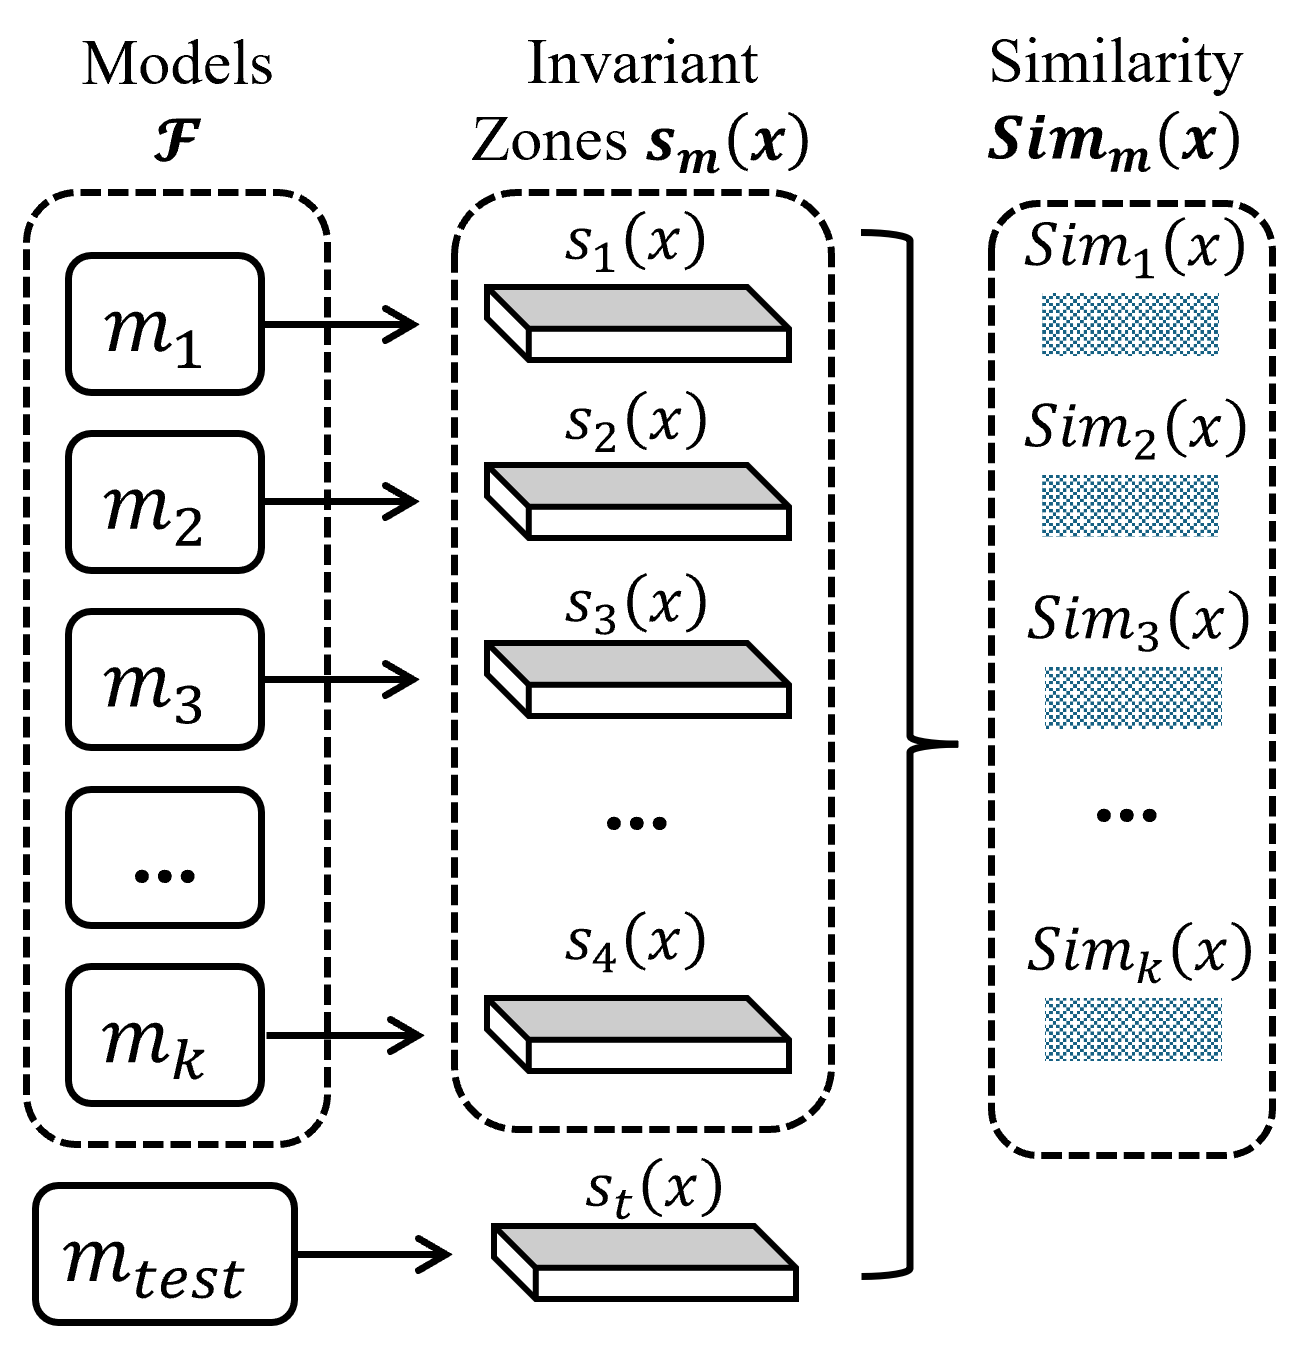
\includegraphics[width=1.0\linewidth]{figures/3_Attribution.png}
  \vspace{-2.0em}
    \caption{
    Zero-shot model attribution via invariant zone signatures. 
    Each model \(m\) is represented by an invariant signature \(s_m(x)\). 
    Given a test model, attribution selects the reference model with highest similarity in invariant space.
    }
    \label{fig:attribution}
  \vspace{-1.5em}
\end{wrapfigure}

The preceding section constructs invariant zones and their corresponding representations \(s_m(x)\), which capture model-specific semantic structure while remaining stable under paraphrasing. We now use these representations for model attribution.

\textbf{Attribution Formulation.}
Let
\(
\mathcal{F}=\{m_1,\ldots,m_K\}
\)
denote a collection of language models. Given an input prompt \(x\), the attribution task is to infer its originating model \(m\in\mathcal{F}\) using invariant zone representations. For each reference model \(m\), we compute its signature \(s_m(x)\), and for a test model we compute \(s_t(x)\). Attribution is then performed by similarity matching
\(
\hat{m}
=
\arg\max_{m\in\mathcal{F}}
\;
\mathrm{Sim}\big(s_t(x),\, s_m(x)\big),
% \label{eq: attibution}
\)
where \(\mathrm{Sim}(\cdot,\cdot)\) denotes a similarity measure such as cosine similarity. 
This formulation corresponds to a zero-shot prototypical~\cite{snell2017prototypical} style classification scheme in invariant representation space, as illustrated in Fig.~\ref{fig:attribution}. Each model is represented by its invariant zone, and attribution is performed by selecting the closest match.

\textbf{Interpretation as Hypothesis Validation.}
Attribution is not posed as a standalone forensic task, but as validation of the proposed geometric framework. If invariant zone representations retain discriminative model identity, this indicates that the discovered invariant structures encode model-specific organization of semantic information. In this way, attribution provides empirical evidence that semantic invariance in language models is a geometric property of latent representations.
